%%%%%%%%%%%%%%%%%%%%%%%%%%%%%%%%%%%%%%%
% Deedy - One Page Two Column Resume
% LaTeX Template
% Version 1.2 (16/9/2014)
%
% Original author:
% Debarghya Das (http://debarghyadas.com)
%
% Original repository:
% https://github.com/deedydas/Deedy-Resume
%
% IMPORTANT: THIS TEMPLATE NEEDS TO BE COMPILED WITH XeLaTeX
%
% This template uses several fonts not included with Windows/Linux by
% default. If you get compilation errors saying a font is missing, find the line
% on which the font is used and either change it to a font included with your
% operating system or comment the line out to use the default font.
% 
%%%%%%%%%%%%%%%%%%%%%%%%%%%%%%%%%%%%%%
% 
% TODO:
% 1. Integrate biber/bibtex for article citation under publications.
% 2. Figure out a smoother way for the document to flow onto the next page.
% 3. Add styling information for a "Projects/Hacks" section.
% 4. Add location/address information
% 5. Merge OpenFont and MacFonts as a single sty with options.
% 
%%%%%%%%%%%%%%%%%%%%%%%%%%%%%%%%%%%%%%
%
% CHANGELOG:
% v1.1:
% 1. Fixed several compilation bugs with \renewcommand
% 2. Got Open-source fonts (Windows/Linux support)
% 3. Added Last Updated
% 4. Move Title styling into .sty
% 5. Commented .sty file.
%
%%%%%%%%%%%%%%%%%%%%%%%%%%%%%%%%%%%%%%%
%
% Known Issues:
% 1. Overflows onto second page if any column's contents are more than the
% vertical limit
% 2. Hacky space on the first bullet point on the second column.
%
%%%%%%%%%%%%%%%%%%%%%%%%%%%%%%%%%%%%%%


\documentclass[]{deedy-resume-openfont}
\usepackage{fancyhdr}
\usepackage{tikzpagenodes}
 
\pagestyle{fancy}
\fancyhf{}
 
\begin{document}

%%%%%%%%%%%%%%%%%%%%%%%%%%%%%%%%%%%%%%
%
%     LAST UPDATED DATE
%
%%%%%%%%%%%%%%%%%%%%%%%%%%%%%%%%%%%%%%
%\lastupdated

%%%%%%%%%%%%%%%%%%%%%%%%%%%%%%%%%%%%%%
%
%     TITLE NAME
%
%%%%%%%%%%%%%%%%%%%%%%%%%%%%%%%%%%%%%%

\begin{tikzpicture}[remember picture,overlay,shift={(current page.north west)}]
\node[anchor=north west,xshift=1.75cm,yshift=-0.25cm]{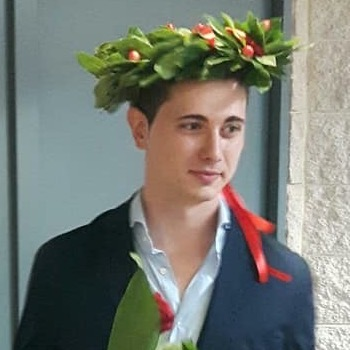
\includegraphics[width=2.5cm]{Foto.jpeg}};
\end{tikzpicture}

\namesection{Massimiliano}{Bruni}{
Email: \href{mailto:massimiliano.bruni@icloud.com}{massimiliano.bruni@icloud.com} | Cell: 334 924 0665
}

%%%%%%%%%%%%%%%%%%%%%%%%%%%%%%%%%%%%%%
%
%     COLUMN ONE
%
%%%%%%%%%%%%%%%%%%%%%%%%%%%%%%%%%%%%%%

\begin{minipage}[t]{0.33\textwidth} 

%%%%%%%%%%%%%%%%%%%%%%%%%%%%%%%%%%%%%%
%     Profilo
%%%%%%%%%%%%%%%%%%%%%%%%%%%%%%%%%%%%%%

\section{Profilo}
Sono un giovane Machine Learning Engineer. Sono appassionato di tecnologia e mi piace lavorare su progetti innovativi. Mi piace realizzare prodotti veri che siano utilizzati da molte persone. Mi piace il lavoro metodico, preciso e con attenzione ai dettagli. Sono diligente, alacre e diplomatico.
\sectionsep

%%%%%%%%%%%%%%%%%%%%%%%%%%%%%%%%%%%%%%
%     Link
%%%%%%%%%%%%%%%%%%%%%%%%%%%%%%%%%%%%%%

\section{Link} 
Github://\href{https://github.com/Maxinho96}{\bf Maxinho96} \\
LinkedIn://\href{https://www.linkedin.com/in/massimiliano-bruni-352926120}{\bf Massimiliano Bruni} \\
YouTube://\href{https://www.youtube.com/channel/UCqskrALDsaUvYC8ztJyqCug}{\bf Massimiliano Bruni} \\
Skype://\href{https://join.skype.com/invite/w9MIsgXZsji7}{\bf live:.cid.52cf21b3deb3210a}
\sectionsep

%%%%%%%%%%%%%%%%%%%%%%%%%%%%%%%%%%%%%%
%     Lingue
%%%%%%%%%%%%%%%%%%%%%%%%%%%%%%%%%%%%%%

\section{Lingue}
\textbf{Italiano}: Madrelingua \\
\textbf{Inglese}: Livello intermedio (B2)
\sectionsep

%%%%%%%%%%%%%%%%%%%%%%%%%%%%%%%%%%%%%%
%     Competenze
%%%%%%%%%%%%%%%%%%%%%%%%%%%%%%%%%%%%%%

\section{Competenze}

\subsection{Hard Skills}
\textbf{Avanzato:} Machine Learning \textbullet{} NLP \\
Python \textbullet{} Pandas \\
\textbf{Intermedio:} Java \textbullet{} SQL \textbullet{} Keras \\
TensorFlow \textbullet{} Scikit-learn \textbullet{} OpenCV \\
Matplotlib \textbullet{} NumPy \textbullet{} Git \textbullet{} Linux \textbullet{} macOS \\
\textbf{Base:} AWS \textbullet{} Hadoop \textbullet{} Spark
\sectionsep

\subsection{Soft Skills}
\textbf{Problem solving}, grazie agli studi in Ingegneria. \\
\textbf{Lavoro in team}, grazie ai vari progetti universitari e di stage. \\
\textbf{Capacità comunicative}, grazie ad una esperienza come tutor privato ed una come studente assistente bibliotecario.
\sectionsep

%%%%%%%%%%%%%%%%%%%%%%%%%%%%%%%%%%%%%%
%     Esami rilevanti
%%%%%%%%%%%%%%%%%%%%%%%%%%%%%%%%%%%%%%

\section{Esami rilevanti}
\textbf{Intelligenza Artificiale}: 30 e lode \\
\textbf{Machine Learning}: 30 e lode \\
\textbf{Sistemi Intelligenti per Internet}: 30 e lode \\
\textbf{Big Data}: 28 \\
\textbf{Analisi e Gestione dell'informazione su web}: 30
\sectionsep

%%%%%%%%%%%%%%%%%%%%%%%%%%%%%%%%%%%%%%
%     Hobby
%%%%%%%%%%%%%%%%%%%%%%%%%%%%%%%%%%%%%%

\section{Hobby}
Sport \textbullet{} Notizie di tecnologia \textbullet{} Videogiochi \\
Giochi da tavolo \textbullet{} Manga

%%%%%%%%%%%%%%%%%%%%%%%%%%%%%%%%%%%%%%
%
%     COLUMN TWO
%
%%%%%%%%%%%%%%%%%%%%%%%%%%%%%%%%%%%%%%

\end{minipage}
\hfill
\begin{minipage}[t]{0.66\textwidth} 

%%%%%%%%%%%%%%%%%%%%%%%%%%%%%%%%%%%%%%
%     Esperienze
%%%%%%%%%%%%%%%%%%%%%%%%%%%%%%%%%%%%%%

\section{Esperienze}

\subsection{Askdata}
\descript{Machine Learning Engineer}
\location{Settembre 2020 - presente | Roma}
Sviluppo modelli di Machine Learning in ambito NLP: Text Summarization, Machine Translation, Named Entity Recognition, Word Similarity. \\
Tecnologie: \textbf{Python} \textbullet{} \textbf{Pandas} \textbullet{} \textbf{Huggingface} \textbullet{} \textbf{SpaCy} \textbullet{} \textbf{Gensim} \textbullet{} \textbf{NLTK}
\sectionsep

\subsection{Istituto di Scienze e Tecnologie della Cognizione - CNR}
\descript{Tirocinante in Machine Learning e Computer Vision}
\location{Marzo 2018 - Luglio 2018 | Roma}
Tirocinio svolto nell'ambito della Tesi Triennale e collegato al progetto descritto sotto chiamato \textit{Robot che riconosce oggetti}. \\
Tecnologie: \textbf{Python} \textbullet{} \textbf{TensorFlow} \textbullet{} \textbf{Scikit-learn} \textbullet{} \textbf{OpenCV} \textbullet{} \textbf{Matplotlib} \textbullet{} \textbf{Numpy}
\sectionsep

%%%%%%%%%%%%%%%%%%%%%%%%%%%%%%%%%%%%%%
%     Istruzione
%%%%%%%%%%%%%%%%%%%%%%%%%%%%%%%%%%%%%%

\section{Istruzione} 

\subsection{Università degli Studi Roma Tre}
\descript{Laurea Magistrale in Ingegneria Informatica}
\location{Ottobre 2018 - Luglio 2020 | Roma}
\location{Voto: 110 e lode}
\sectionsep

\subsection{Istituto di Scienze e Tecnologie della Cognizione - CNR}
\descript{Advanced School in Artificial Intelligence}
Master in Machine Learning Applications \\
\location{Ottobre 2019 - Aprile 2020 | Roma}
\sectionsep

\subsection{Università degli Studi Roma Tre}
\descript{Laurea Triennale in Ingegneria Informatica}
\location{Settembre 2015 - Luglio 2018 | Roma}
\location{Voto: 110 e lode}
\sectionsep

%%%%%%%%%%%%%%%%%%%%%%%%%%%%%%%%%%%%%%
%     Certificazioni
%%%%%%%%%%%%%%%%%%%%%%%%%%%%%%%%%%%%%%

\section{Certificazioni}
\begin{tabular}{@{}lll@{}}
\textbf{Anno} & \textbf{Ente} & \textbf{Certificato} \\
2017          & Coursera      & \textit{Machine Learning} \\
2015	      & Cambridge     & \textit{B2 First} \\
2015	      & Cisco         & \textit{CCNA Discovery: Networking for Home and Small Businesses} \\
\end{tabular}
\sectionsep

%%%%%%%%%%%%%%%%%%%%%%%%%%%%%%%%%%%%%%
%     Progetti
%%%%%%%%%%%%%%%%%%%%%%%%%%%%%%%%%%%%%%

\section{Progetti}

\descript{Sistema di videosorveglianza (\href{https://github.com/Maxinho96/person\_identification}{Link})}
Per la Tesi Magistrale ho realizzato un sistema di videosorveglianza che rileva le persone e determina anche le loro identità dato un dataset di persone note.

\descript{Object Detection con drone (\href{https://youtu.be/cnnGjHns818}{Link})}
Per la Advanced School in Artificial Intelligence ho realizzato un sistema di object detection sulla camera di un drone.

\descript{Bot Telegram: classificatore di immagini (\href{https://github.com/Maxinho96/Image-Classifier-Telegram-Bot}{Link})}
Come progetto personale ho realizzato un bot Telegram a cui si può inviare un'immagine per sapere quale oggetto vi è rappresentato.

\descript{Robot che riconosce oggetti (\href{https://github.com/Maxinho96/Machine-Learning-Research-Project}{Link})}
Per la Tesi Triennale ho realizzato un sistema pensato per funzionare su un robot che riconosce oggetti comuni ed impara autonomamente nuovi oggetti.

%%%%%%%%%%%%%%%%%%%%%%%%%%%%%%%%%%%%%%
%     Dati personali
%%%%%%%%%%%%%%%%%%%%%%%%%%%%%%%%%%%%%%

\footnotetext{Autorizzo il trattamento dei dati personali contenuti nel mio curriculum vitae.}

\end{minipage} 
\end{document}  \documentclass[]{article}
